\documentclass[12pt, a4paper]{article}
\usepackage[utf8]{inputenc}
\usepackage[T1]{fontenc}
\usepackage[slovene]{babel}
\usepackage{lmodern}
\usepackage{amsmath}
\usepackage{units}
\usepackage{eurosym}
\usepackage{amsfonts}
\usepackage{fancyhdr,amssymb,amsmath,amsthm,bbm,enumerate,mdwlist,url,multirow,hyperref,graphicx}
\usepackage{pdfpages}
\usepackage{comment}
\usepackage{breqn}
\usepackage{caption}
\usepackage{subcaption}
\usepackage{float}
\usepackage{graphicx}


\usepackage{enumerate}
\setlength{\parindent}{0mm}

\DeclareUnicodeCharacter{2212}{-}

\begin{document}
\begin{titlepage}
\begin{center}

\large
Univerza v Ljubljani\\
\normalsize
Fakulteta za matematiko in fiziko\\

\vspace{5 cm} 

\large
Finančni praktikum \\


\vspace{0.5cm}
\LARGE
\textbf{Stable roommate problem}

\vspace{0.5 cm}

\large
Timotej Giacomelli in Nejc Duščak\\


\vspace{1.5cm}
\normalsize
Mentorja: prof. dr. Sergio Cabello, asist. dr. Janoš Vidali
\vspace{3cm}


\vfill

\large Ljubljana, 2020

\end{center}
\end{titlepage}


\newpage

\tableofcontents
\vspace{22mm}

\newpage

\section{Uvod}
V projektu pri finančnem praktikumu bova obravnavala \textit{Stable roommate problem}.  Problem bova modelirala in poganjala ekspiremente v programskem jeziku Sage.\\

\textit{Stable roommate problem}, znan tudi kot kratica \textbf{SR}, je eden izmed \textit{stable matching} problemov, katere sta prvič predstavila David Gale in Lloyd Shapely. Problem je dobil ime zaradi svoje praktične uporabe - kako razporediti ljudi v dvoposteljne sobe, glede na njihove preference.\\

Problem je sestavljen iz $2n$ "udeležencev", kjer ima vsak udeleženec seznam preferenc s $2n - 1$ elementi, torej po eno vrednost za vsakega soudeleženca. Vsak udeleženec predstavljen točko v metričnem prostoru, njegov seznam pa so urejene dolžine do ostalih soudeležencev.\\

Ujemanje je množica $n$ disjunktnih parov udeležencev.
Za ujemanje $M$ je par $\{m_{1}, m_{1}' \} \notin M$ \textit{blocking pair}, če zadošča naslednjim pogojem:
\begin{itemize}
	\item  $\{m_{1}, m_{1}' \}, \{m_{2}, m_{2}' \} \in M$,
	\item $m_1$ preferira $m_2$ bolj kot $m_1'$,
	\item $m_2$ preferira $m_1$ bolj kot $m_2'$.
\end{itemize}
Oziroma če povemo z besedami, \textit{blockin pair} nastane, če se imata vsaj dva udeleženca, ki nista v paru, pri ujemanju raje, kot s svojim partnerjem.
Ujemanje $M$ je nestabilno, če zanj obstaja \textit{blocking pair}. Drugače je ujemanje $M$ stabilno.\\

Cilj SR je najti stabilno ujemanje ali pokazati, da nobeno ne obstaja. S časoma so uspeli razviti algoritem s časovno zahtevnostjo $O(n^2)$, ki bodisi najde stabilno ujemanje, bodisi ugotovi, da za dani primer ne obstaja nobeno stabilno ujemanje.\\

Stable roommate problem je v splošnem lahko uporabljen za ujemanje opazovanj in objektov pri nalogi razvrščanja. Na primer v življenjskem primeru iskanje primernega sostanovalca, so lahko le-ti predstavljeni po točkah v nekem prostoru lastnosti: koordinatna os prostora je lahko najprimernejši čas za spanje, želena raven urejenosti prostora, število zabav/piv na semester, itd.. Povsem logično je sklepati, da bo izbran udeleženec tisti, ki bo imel podobne lastnosti. \\

\pagebreak
V nadaljevanju projekta bova sledeila sledečim korakom:
\begin{itemize}
	\item generirala bova $2n$ naključnih točk v kvadratu velikosti 1x1,
	\item izračunala bova posamezne razdalje med točkami,
	\item razdalje bodo predstavljale najine preference (manjša razdalja je večja preferenca), ki jih bova uredila po velikosti,
	\item napisala bova algoritem, ki bo izračunal ujemanje ali pa ugotovil, da ujemanje ne obstaja,
	\item analizirala bova, ali se seštevek razdalj med točkami v paru povečuje, ali zmanjšuje, ko povečujeva število točk ($n$).
\end{itemize}

\newpage

\section{Opis problema}
\textit{Stable roomate problem} je problem v katerem želimo poiskati stabilno ujemanje udeležencev v problemu. Vsak udeleženec ima seznam preferenc do drugih udeležencev. Seznam je urejen po velikosti od najvišje preference pa vse do najnižje. Če bi želeli problem predstaviti v realnosti, si lahko mislimo, da imamo posameznika, ki si želi poiskati sostanovalca. Glede na njegove želje bo potencialne sostanovalce uredil glede na svoje preference in nato izbral posameznika z najvišjo preferenco.\\
V projektu pa sva obravnavala enostavnejšo verzijo osnovnega problema, in sicer \textit{Geometric stable roomate problem}. V tem problemu so udeleženci predstavljeni kot točke v ravnini, kjer lahko te točke izberemo iz poljubno omejenega območja ali pa točke izbiramo kar iz celotne ravnine. V najinem projektu sva točke izbrala iz kvadrata velikosti 1x1. Preference so tukaj zelo preproste, saj so podane le kot razdalja do točk. Tako manjša razadlja do točke pomeni večjo preferenco. V tem problemu želiva poiskati stabilne pare, ki ustrezajo seznamu preferenc. \\

\begin{center}
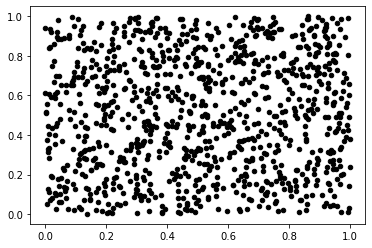
\includegraphics{rdece_tocke.png}
\end{center}


\pagebreak
\section{Glavne ideje problema in psevdokoda}
Za iskanje rešitev problema sva si izbrala poljubne točke znotraj kvadrata velikosti 1x1. Generirala sva x in y koordinato posamezne točke in jih shranila v \textit{slovar točk}, kjer ključ slovarja predstavljajo ime točke (naprimer \textit{tocka_0}), vrednost pa koordinata točke. Vrednost slovarja je oblike (\textit{x,y}) kar imenujemo tupli. V nadaljevanju projekta bova poskusila točke izbirati tudi iz območij drugačne oblike, če bo le možno tudi točke iz neomejenega območja.\\

Nato sva izračunala razdalje med točkami s pomočjo Pitagorovega izreka. S funkcijo \textit{for} sva se sprehodila čez vse ključe v \textit{slovarju točk} in oblikovala novi slovar imenovan \textit{slovar razdalj}, v katerem je ključ slovarja ponovno ime točke, vrednost pa vsebuje seznam razdalj do posamezne točke, torej dobimo seznam tulpov. Prvotno sva računanje Pitagorovega izreka  razdelila na 3 podprimere. Kasneje sva našla hitrejši način, ki za izračun razdalje porabi manj časa. V nadaljevanju sva s pomočjo funkcije \textit{preference} uredila \textit{slovar razdalj} glede na razdaljo. Tako sva dobila seznam tulpov, urejen po velikosti od najkrajše do najdaljše razdalje.  \\

Do sedaj sva zgenerirala slovar v katerem imava vse točke in urejen seznam preferenc.  V tem delu projekta pa nastopi reševanje problema. Ideja reševanja problema je bila, da bi se sprehodila čez vse točke v slovarju in pri vsaki točki preverila njene preference. Ko bi našla najkrajšo razdaljo med dvema točkama, bi ti dve točki povezala v par in posledično na koncu pridobila ujemajoče pare. Algoritem za reševanje te ideje pa sva sestavila iz dveh funkcij:
\begin{itemize}
	\item prvo sva sestavila funkcijo \textit{Najkrajsa}, ki poišče najkrajšo razdaljo med vsemi točkami. Sprehodimo se po vseh točkah in preverimo njihove prve preference. Ko najdemo najmanjšo oziroma najkrajšo razdaljo, funkcija izbere tisti dve točki, med katerima ta razdalja nastopi in ju poveže v par. Na koncu nam vrne par točk, s pripadajočo najmnajšo razdaljo,
	\item druga funkcija pa se imenuje \textit{Vsi_pari}, ki nam omogoča, da kličemo funkcijo \textit{Najkrajsa} dokler ne povežemo vse točke v paru. Pomembno je tudi omeniti, da ko najdemo povezavo med dvema točkamo, potem ti dve točki izbrišemo iz seznama preferenc drugih točk, saj tako dosežemo, da se funkcija hitreje konča.
\end{itemize}

\pagebreak
\section{Reševanje problema izenačenja}
Pri pregledu pravilnosti reševanja problema sva ob koncu naletela na problem izenačenja. Nastopi, ko pride do pojava, ko ima poljubna točka enako razdaljo do dveh drugih točk v ombočju. To pomeni, da ima enako preferenco do dveh točk. Najin algoritem pri uporabi funkcije \textit{preference} uredi razdaljo po velikosti, če pa se pojavi problem izenačenja pa kot prvo točko navede tisto, ki je prva ko se funkcija sprehodi skozi ključe \textit{slovarja razdalj}. Zato kasneje, ko pridemo do reševanja problema s funkcijama \textit{Najkrajsa} in \textit{Vsi_pari} naletimo na problem, ko funkciji pogledata le prvo preferenco, ne upoštevata pa možnost izenačenja. Tako sva bila primorana algoritem prilagoditi tudi za primer izenačenja. \\

\pagebreak
\section{Eksperimentiranje z algoritmom}
Za eksperimentiranje z najinim algoritmom sva si izbrala računanje vsote razdalj med točkami v izbranem območju in preverila kako se vsota obnaša glede na število točk, ki jih izbereva, in glede na območje, ki sva ga izbrala. Za ta namen sva sestavila funkciji \textit{vsota_razdalj} in \textit{razlicne_vsote}. Funkcija  \textit{vsota_razdalj} izračuna razdaljo med vsemi točkami, ki nostopajo v paru, tako da po vrsti gleda razdalje točk v paru in jih sešteva. Funkcijo \textit{razlicne_vsote} pa sva sestavila z namenom, da opazujeva eksperiment in sicer naju je zanimalo, kako se vsote obnašajo, ko povečujemo število točk. \\
\subsection{Eksperimentiranje v kvadratu velikosti 1x1}
Pri opazovanju gibanja števila vsote sva dobila spodnjo funkcijo.\\
\begin{center}
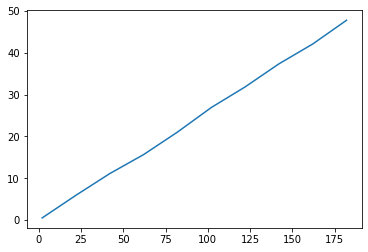
\includegraphics{kvadrat_1x1.png}
\end{center}
Lahko opazimo, da vsote naraščajo skupaj s številom točk. Seveda v nekaterih primerih prihaja do manjših odstopanj, vendar je opazno, da vsote rastejo.

\subsection{Eksperimentiranje v krogu s polmerom r}
V drugem primeru sva definirala točke znotraj kroga s polmerom r, kjer sva polmer r izbrala na začetku. Tu lahko eksperimentiramo na več različnih načinov:
\begin{itemize}
	\item povečujemo število izbranih točk pri dani izbiri r=1
\begin{center}
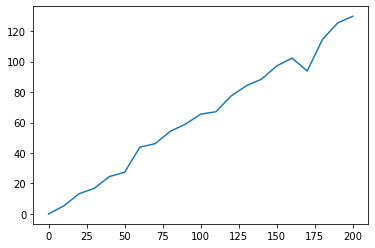
\includegraphics{krog_s_danim_polmerom.png}
\end{center}
Opazimo, da tudi v tem primeru vsote rastejo enakomerno z višanjem števila izbranih točk.

	\item povečujemo r pri dani izbiri n=10

	
\end{itemize}

\newpage

\subsection{Eksperimentiranje s kvadratom in krogom}
V tem razdelku, bi rada opazovala kako različna območja (v najinem primeru kvadrat in krog), ki imajo enako površino, vplivajo na vsoto razdalj vseh točk v paru. Za ta primer sva si izbrala kvadrat velikosti 1x1, na drugi strani pa sva izbrala krog s polmerom r=1/sqrt(pi). Tako sva dobila območji, ki imata enako ploščino. Sedaj bomo lahko videli ali oblika območja vpliva na vsoto.\\
\begin{center}
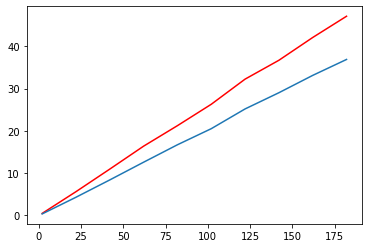
\includegraphics{primerjava_krog_kvadrat.png}
\end{center}
Na sliki so z rdečo barvo označene vsote točk, ki ležijo v kvadratu, z modro pa točke, ki ležijo v krogu. Opazimo lahko, da so vsote večje v krogih kot v kvadratih.\\
Če pa pogledamo še spodnjo sliko pa lahko še bolj nazorno opazimo, da vsote točk v krogu tudi hitreje naraščajo.
\begin{center}
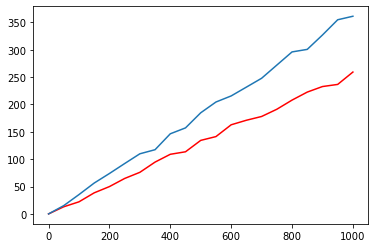
\includegraphics{primerjava_krog_kvadrat_2.png}
\end{center}


\end{document}